\documentclass[12pt,fleqn,a4paper,oneside]{LegrandOrangeBook}
\addbibresource{sample.bib} % Bibliography file
\definecolor{ocre}{RGB}{103, 61, 76}
\chapterimage{orange1.jpg} 
\chapterspaceabove{6.5cm}
\chapterspacebelow{6.75cm} 
%\begin{theorem}[Name of the theorem]
%\begin{exercise}
%\begin{example}[Example name]
%\begin{definition}[Definition name]
%\begin{corollary}[Corollary name]
%\begin{remark}
%\begin{proposition}[Proposition name]
%\begin{problem}
%\begin{vocabulary}[Word]
%\begin{notation}
%----------------------------------------------------------------------------------------
\begin{document}
%----------------------------------------------------------------------------------------
%----------------------------------------------------------------------------------------
%	NEW CHAPTER
%----------------------------------------------------------------------------------------
%\part{Legislación y regulación}
%\chapterimage{chapter_head_LR.pdf} % Chapter heading image
%
%\part{Proyecto final 1}
%\chapterimage{chapter_head_PF1.pdf} % Chapter heading image
%
%
%\part{Dispositivos de fibra óptica}
%\chapterimage{chapter_head_FO.pdf} % Chapter heading image
%\chapter{Transmisores ópticos}
%Para los dos tipos de transmisores ópticos tenemos:
%\begin{itemize}
%\item \textbf{LED}: Usado para fines multimodo.
%\begin{enumerate}
%\item Superficial (SLED)
%\item Borde o lateral (ELED)
%\item Superluminiscente o superradiante (SLD)
%\end{enumerate}
%
%\item \textbf{Láser}: Usado para fines monomodo.
%\begin{enumerate}
%\item Multimodo
%\begin{itemize}
%\item Fabri-Perot
%\end{itemize}
%\item Monomodo
%\begin{itemize}
%\item DBR
%\item DFB
%\item VC-SEL\footnote{Principalmente en aplicaciones multimodo, aunque también puede ser adaptarse a aplicaciones monomodo bajo ciertas condiciones y requisitos específicos.}
%\end{itemize}
%\end{enumerate}
%\end{itemize}
%\begin{figure}[H]
%\centering
%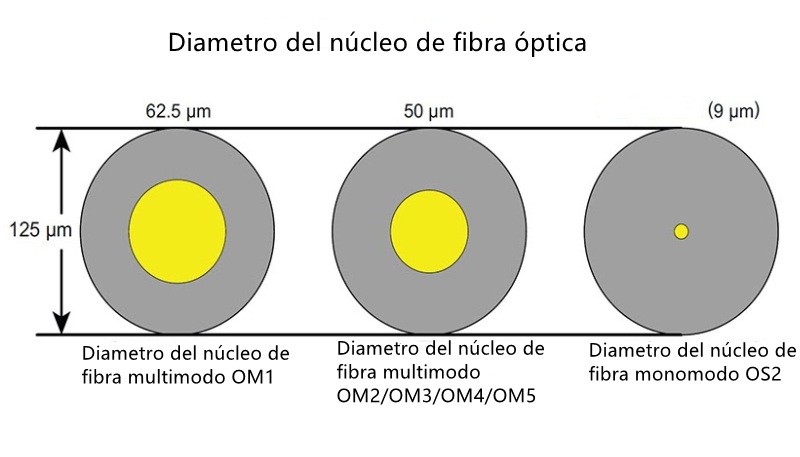
\includegraphics[width=0.7\linewidth]{Dfo/dfo1.png}
%\caption{Diámetro de núcleo de fibra óptica.}
%\end{figure}
%Algunas \textbf{generalidades} antes de continuar:
%\begin{itemize}
%\item Diodos semiconductores elaborados con materiales de los grupos III, IV, V y VI de la tabla periódica:
%\begin{itemize}
%\item III: Galio (Ga), Boro (B), Aluminio (Al) y Indio (In)
%\item IV: Plomo (Pb) y Estaño (Sn).
%\item V: Arsénico (), Fósforo (P), Antimonio (Sb) y Bismuto (Bi).
%\item VI: Azufre (S), Selenio (Se) y Telurio (Te).
%\end{itemize}
%\item Tipos de emisión de luz:
%\begin{itemize}
%\item Emisión Espontánea: En la emisión espontánea, los electrones en un material emisor de luz se relajan de un estado de energía más alto a uno más bajo, liberando energía en forma de fotones. Esta emisión ocurre de manera aleatoria y no está sincronizada. Por ejemplo, la emisión espontánea ocurre en la mayoría de los materiales luminiscentes convencionales, como los materiales fluorescentes.
%\item Emisión Estimulada: En la emisión estimulada, los electrones son estimulados para liberar fotones adicionales al interactuar con fotones incidentes. Este proceso es el principio fundamental detrás de los láseres y los amplificadores ópticos. La emisión estimulada se caracteriza por ser coherente y tener una fase y dirección bien definidas.
%\end{itemize}
%\end{itemize}
%\section{LED}
%También tenemos que recordar las características generales de los diodos LED:
%\begin{enumerate}
%\item Reducido tamaño y peso: Los diodos LED son dispositivos compactos y livianos, lo que facilita su integración en diversos diseños y aplicaciones.
%\item Superficies radiantes compatibles en tamaño: Los diodos LED tienen una superficie radiante que emite luz, y esta superficie se adapta a diferentes tamaños según el tipo y el modelo del LED.
%\item Fácil modulación: Los diodos LED pueden ser modulados fácilmente para variar su brillo o encendido y apagado rápidamente, lo que permite su uso en aplicaciones de señalización y comunicación.
%\item Bajo consumo de corriente: Los diodos LED requieren un consumo de corriente eléctrica relativamente bajo para emitir luz, lo que los hace eficientes en términos de consumo de energía.
%\item Alta velocidad de respuesta: Los diodos LED tienen una alta velocidad de respuesta, lo que significa que pueden encenderse y apagarse rápidamente en cuestión de nanosegundos.
%\item Espectro de emisión coincidente con la ventana de $T_x$: Esta característica se refiere a que los diodos LED emiten luz en un rango de longitud de onda que es compatible con la ventana de transmisión de un sistema de comunicación óptica.
%\item Reducido anchura espectral: Los diodos LED emiten luz en un rango de anchura espectral relativamente estrecho, lo que significa que la luz emitida se concentra en una estrecha banda de longitud de onda.
%\item Estrecho lóbulo de emisión: Los diodos LED tienen un lóbulo de emisión direccional estrecho, lo que significa que la luz se emite en una dirección específica, lo que facilita el direccionamiento y la concentración de la luz en una región deseada.
%\item Alta potencia óptica de salida: Los diodos LED pueden proporcionar una potencia óptica de salida significativa, lo que significa que pueden emitir una cantidad considerable de luz en comparación con su tamaño y consumo de energía.
%\item Características estables (usar climatizador): Para garantizar un rendimiento óptimo, algunos diodos LED pueden requerir un control preciso de la temperatura, lo cual se puede lograr utilizando un climatizador o dispositivos de enfriamiento adecuados.
%\end{enumerate}
%\begin{figure}[H]
%\centering
%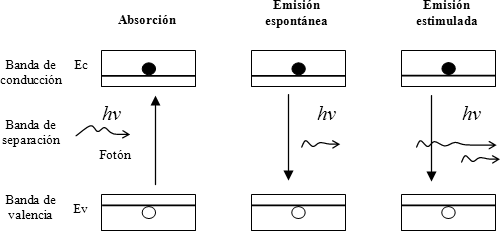
\includegraphics[width=\linewidth]{Dfo/dfo2.png}
%\caption{Conversión eléctrica.}
%\end{figure}
%\begin{enumerate}
%\item \textbf{Absorción}: La absorción es el proceso mediante el cual un material absorbe energía lumínica. Cuando un fotón interactúa con un átomo, molécula o material semiconductor, puede transferir su energía al sistema, lo que resulta en la excitación de los electrones del material a niveles de energía más altos. Como resultado, el fotón es absorbido y su energía se convierte en energía interna del material. La absorción se produce cuando la energía del fotón coincide con la diferencia de energía entre los niveles de energía permitidos en el material.
%\begin{itemize}
%\item En ingeniería fotovoltaica, los paneles solares absorben la energía de la luz solar y la convierten en electricidad.
%\item En fibra óptica, los cables de fibra óptica utilizados para transmitir señales de datos absorben la luz y la guían a lo largo de la fibra.
%\end{itemize}
%\item \textbf{Emisión espontánea}: La emisión espontánea ocurre cuando los electrones excitados en un material emisor de luz se relajan de un estado de energía más alto a uno más bajo sin ninguna influencia externa. Durante este proceso, el electrón emite un fotón y regresa a su estado de energía original. La emisión espontánea es aleatoria y no está sincronizada, lo que significa que los fotones emitidos tienen diferentes direcciones de propagación y fases. Este fenómeno es común en muchos materiales luminiscentes, como los materiales fluorescentes, donde los electrones excitados se desexcitan espontáneamente y emiten fotones de luz.
%\begin{itemize}
%\item En la iluminación LED, los diodos emisores de luz emiten fotones cuando los electrones se relajan de niveles de energía más altos a niveles de energía más bajos de manera espontánea.
%\item En los dispositivos de visualización, como las pantallas OLED, la emisión espontánea se utiliza para generar luz y mostrar imágenes.
%\end{itemize}
%\item \textbf{Emisión estimulada}: La emisión estimulada es un proceso en el cual un electrón excitado en un material emisor de luz es inducido a decaer a un nivel de energía más bajo mediante la interacción con un fotón incidente. En este caso, el fotón incidente tiene una energía y una dirección específicas que coinciden con las características del electrón excitado. Cuando el fotón interactúa con el electrón excitado, el electrón se desexcita y emite un segundo fotón con la misma energía, fase y dirección que el fotón incidente. A diferencia de la emisión espontánea, la emisión estimulada es un proceso determinista y está sincronizada con la presencia del fotón incidente. Este proceso es la base del funcionamiento de los láseres y amplificadores ópticos, donde se utiliza un medio activo para lograr la emisión estimulada y generar luz coherente y direccional.
%\begin{itemize}
%\item En los láseres, se utiliza la emisión estimulada para generar luz coherente y direccional. Un fotón incidente estimula la emisión de más fotones idénticos, lo que amplifica la luz y la hace coherente.
%\item En la amplificación óptica de señales, como en los amplificadores ópticos de fibra, se utiliza la emisión estimulada para amplificar una señal óptica débil mediante la interacción con fotones de una fuente de bombeo.
%\end{itemize}
%\end{enumerate}
%\begin{figure}[H]
%\centering
%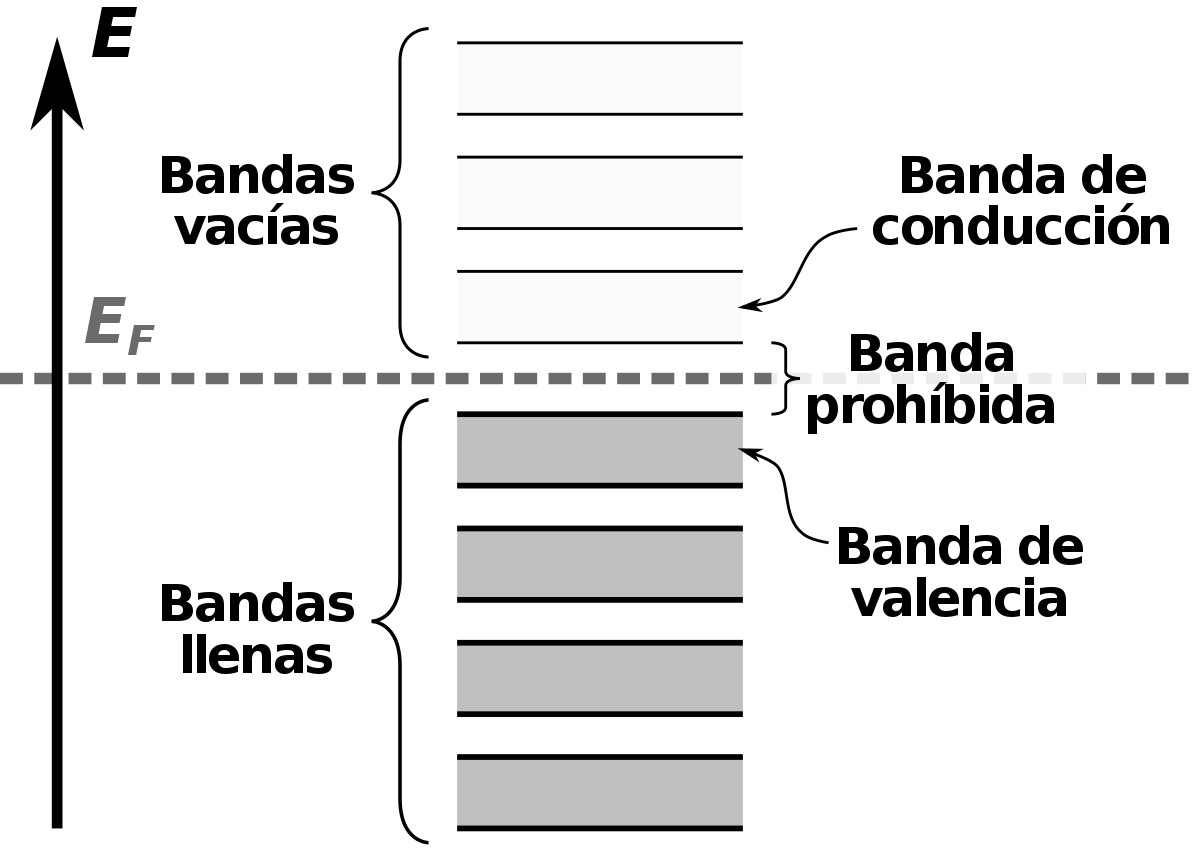
\includegraphics[width=0.7\linewidth]{Dfo/dfo3.png}
%\caption{Bandas de energía.}
%\end{figure}
%\begin{definition}[Energía Gap]
%La energía de la banda prohibida o energía gap ($E_g$) de un material semiconductor se puede calcular utilizando la ecuación de la relación entre la energía de un fotón y su longitud de onda. La ecuación es la siguiente:
%\begin{equation}
%E_g=\frac{h\cdot c}{\lambda}
%\label{eq:energiaGap}
%\end{equation}
%Donde:
%\begin{itemize}
%\item $E_g$: Es la energía de la banda prohibida o energía gap del material. (eV)
%\item $h$ La constante de Planck (aproximadamente $6.626\basedec{-34} J\cdot s $  o $4.136\basedec{-15} eV\cdot s$).
%\item \textbf{c}: Es la velocidad de la luz en el vacío (aproximadamente $3\basedec{8}m/s$). (m/s)
%\item $\lambda$: Longitud de onda de la luz incidente en el material. (m)
%\end{itemize}
%\end{definition}
%\begin{notation}
%Para apreciar los colores de manera más precisa y natural, se recomienda utilizar una fuente de luz que tenga un espectro continuo y equilibrado. Tanto la luz solar como algunas fuentes de luz incandescentes, como las lámparas halógenas, proporcionan un espectro completo y pueden permitir una buena representación de los colores.
%\end{notation}
%\subsection{Tipos de estructuras de los diodos LED}
%%Imagen de diodo  led
%\subsubsection{LEDs de superficie-SLED}
%Para lograr el acoplamiento eficiente entre un LED de superficie y una fibra óptica, se aprovecha la radiación que emerge desde un plano paralelo al de la unión semiconductora. Esta radiación se emite en forma de un cono de luz divergente. El LED de superficie está diseñado de tal manera que la región emisora de luz se encuentra en un plano paralelo al plano de unión semiconductora. Esto permite que la luz emitida se propague en un amplio ángulo con respecto al eje óptico del LED. Esta configuración es diferente de los LED convencionales, donde la emisión se produce principalmente en un ángulo estrecho y perpendicular al plano de la unión. Cuando se coloca una fibra óptica cerca del LED de superficie, el cono de luz emitido por el LED se acopla en la abertura de entrada de la fibra óptica. La geometría de la fibra óptica está diseñada para captar la mayor cantidad posible de luz emitida por el LED y guiarla a lo largo de la fibra. El acoplamiento eficiente se logra al optimizar el ángulo de inclinación y la posición relativa entre el LED de superficie y la fibra óptica. Además, se utilizan técnicas de alineación precisa y lentes ópticas para enfocar y mejorar la captación de la luz emitida por el LED.
%\subsubsection*{LED de emisión superficial: tipo burrus}
%\begin{figure}[H]
%\centering
%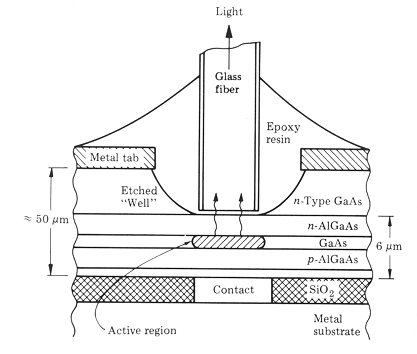
\includegraphics[width=0.5\linewidth]{Dfo/dfo5.png}
%\caption{Led superficial: Burrus .}
%\end{figure}
%A diferencia de los diodos de unión PN convencionales, que tienen una unión PN en el interior del semiconductor, los diodos de superficie tipo Burrus tienen una \textbf{estructura de barrera} de superficie en la interfaz entre el metal y el semiconductor. Para evitar la absorción de la radiación óptica en la capa \textit{n}, se usan estructuras de capas muy estrechas, tallandose una abertura cóncava en la capa \textit{n}, que permite alojar el extremo de la fibra, aproximadamente a la capa \textit{p}, que es donde se produce la emisión luminosa consiguiendo una \textbf{alta radiancia}.\\
%Esta estructura de barrera de superficie proporciona varias ventajas en comparación con los diodos de unión PN convencionales. Algunas de estas ventajas incluyen:
%\begin{enumerate}
%\item \textbf{Velocidad de conmutación rápida}: Los diodos de superficie tipo Burrus tienen una estructura de barrera de superficie que permite una respuesta más rápida y una mayor velocidad de conmutación. Esto los hace adecuados para aplicaciones de alta frecuencia y alta velocidad, como en circuitos de radiofrecuencia y comunicaciones.
%\item \textbf{Baja capacitancia}: La estructura de barrera de superficie reduce la capacitancia del diodo, lo que resulta en una menor carga y descarga de la corriente en aplicaciones de alta frecuencia.
%\item \textbf{Baja distorsión armónica}: Debido a su diseño especial, los diodos de superficie tipo Burrus tienen una baja distorsión armónica, lo que los hace adecuados para aplicaciones en las que se requiere una alta calidad de señal y una baja distorsión, como en equipos de audio y comunicaciones de alta fidelidad.
%\end{enumerate}
%\subsubsection*{Diodo Burrus con Heterounión}
%\begin{figure}[H]
%\centering
%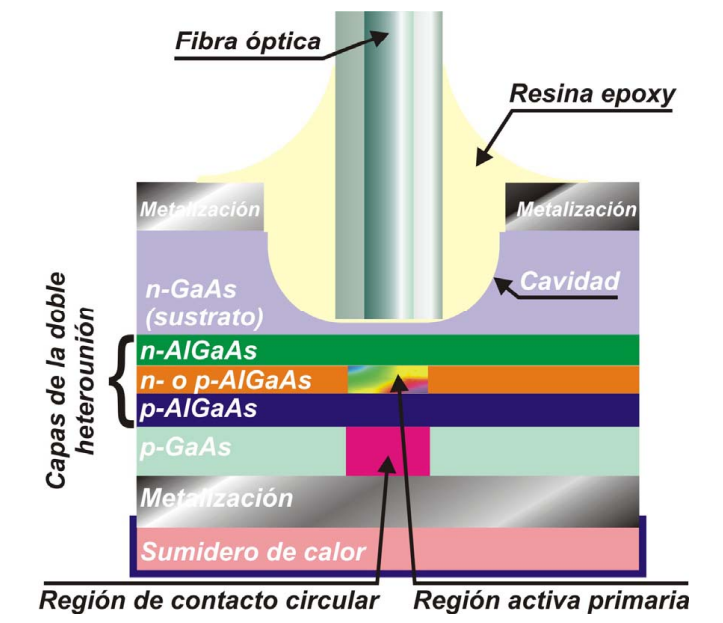
\includegraphics[width=0.5\linewidth]{Dfo/dfo4.png}
%\caption{Led superficial: Burrus y heterounión.}
%\end{figure}
%La radiancia de un LED de superficie es del orden de $2W/sr.cm^2$\footnote{La radiancia ser mide en "Vatio por metro cuadrado por esteroradián".} para una corriente de unos 200mA, pero estos valores pueden mejorarse hasta $50W/sr.cm^2$. La caracteristica de radiación de un LED de superficie es de tipo \textbf{Lambertiano} (coseno), es decir, la potencia emitida según un determinado ángulo $\theta$ respecto a al normal de la superficie emisora es:
%\begin{equation}
%P(\theta)=P_0\cdot\cos\theta
%\end{equation}
%Donde:
%\begin{itemize}
%\item $P(\theta)$: Potencia emitida por el LED en un ángulo $\theta$. (W).
%\item $P_0$: Potencia total emitida por el LED sin considerar el ángulo sólido. (W).
%\item $I(\theta)$: Función de distribución angular, que representa la intensidad luminosa en función del ángulo $\theta$.  (W/sr).
%\item $\theta$: Ángulo sólido formado con el eje x. (sr)\footnote{Esteroradián.}.
%\end{itemize}
%\subsubsection{Diodo led de borde-ELED}
%Los LEDs de emission lateral o de borde (edge-emitting LEDs o ELED) surgieron como desarrollo posterior ante la demanda de fuentes que pudiesen alcanzar mayor distancia, a mayor longitud de onda y con mayor tasa binaria. En los ELED, la región activa es una tira estrecha que se crea bajo la superficie del sustrato. Éste se corta o se pule de manera que la tira alcanza los dos extremos del dispositivo. Se emplea una doble heteroestructura con los mismos fines que en los SLED, y además como
%guiaonda, haciendo el índice de la zona activa superior al de las dos zonas inmediatas. También se confina lateralmente. La faceta trasera se suele tallar o recubrir para hacerla reflectante, mientras que la delantera, por donde se produce la salida del haz de luz, se recubre de un material antirreflexivo. De este modo se optimiza la salida a un solo borde.
%Los ELED son capaces de acoplar mayor porcentaje de potencia que los SLED a fibras con baja apertura numérica. En algunas aplicaciones se utilizan asociados a fibras monomodo. El rango espectral de la emisión es asimismo más estrecho en los ELED. Como contrapartida, los ELED son más sensibles a los cambios de temperatura que los SLED.
%\begin{figure}[H]
%\centering
%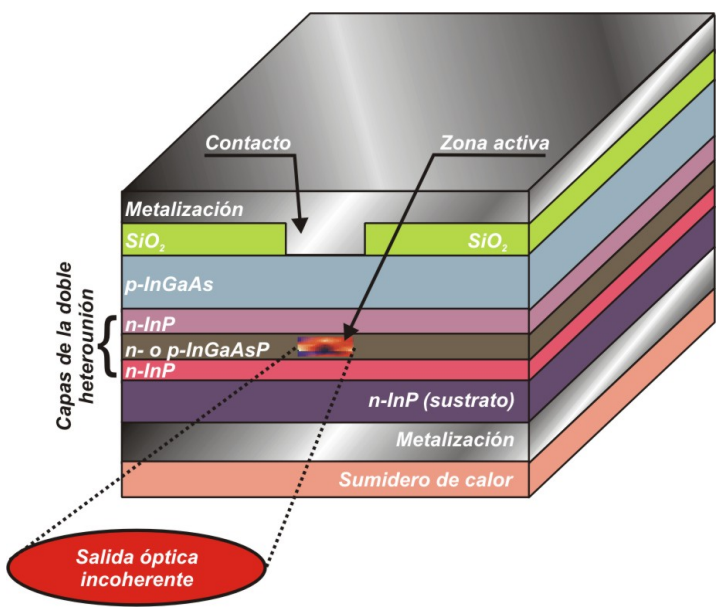
\includegraphics[width=0.6\linewidth]{Dfo/dfo6.png}
%\caption{LED de emisión lateral.}
%\end{figure}
%En este caso la distribución enérgetica no es del tipo Lambertiano, como ocurre en los LED de superficie, sino aparece como un lóbulo de radiación de sección transversal en cierto modo elíptica.
%\begin{figure}[H]
%\centering
%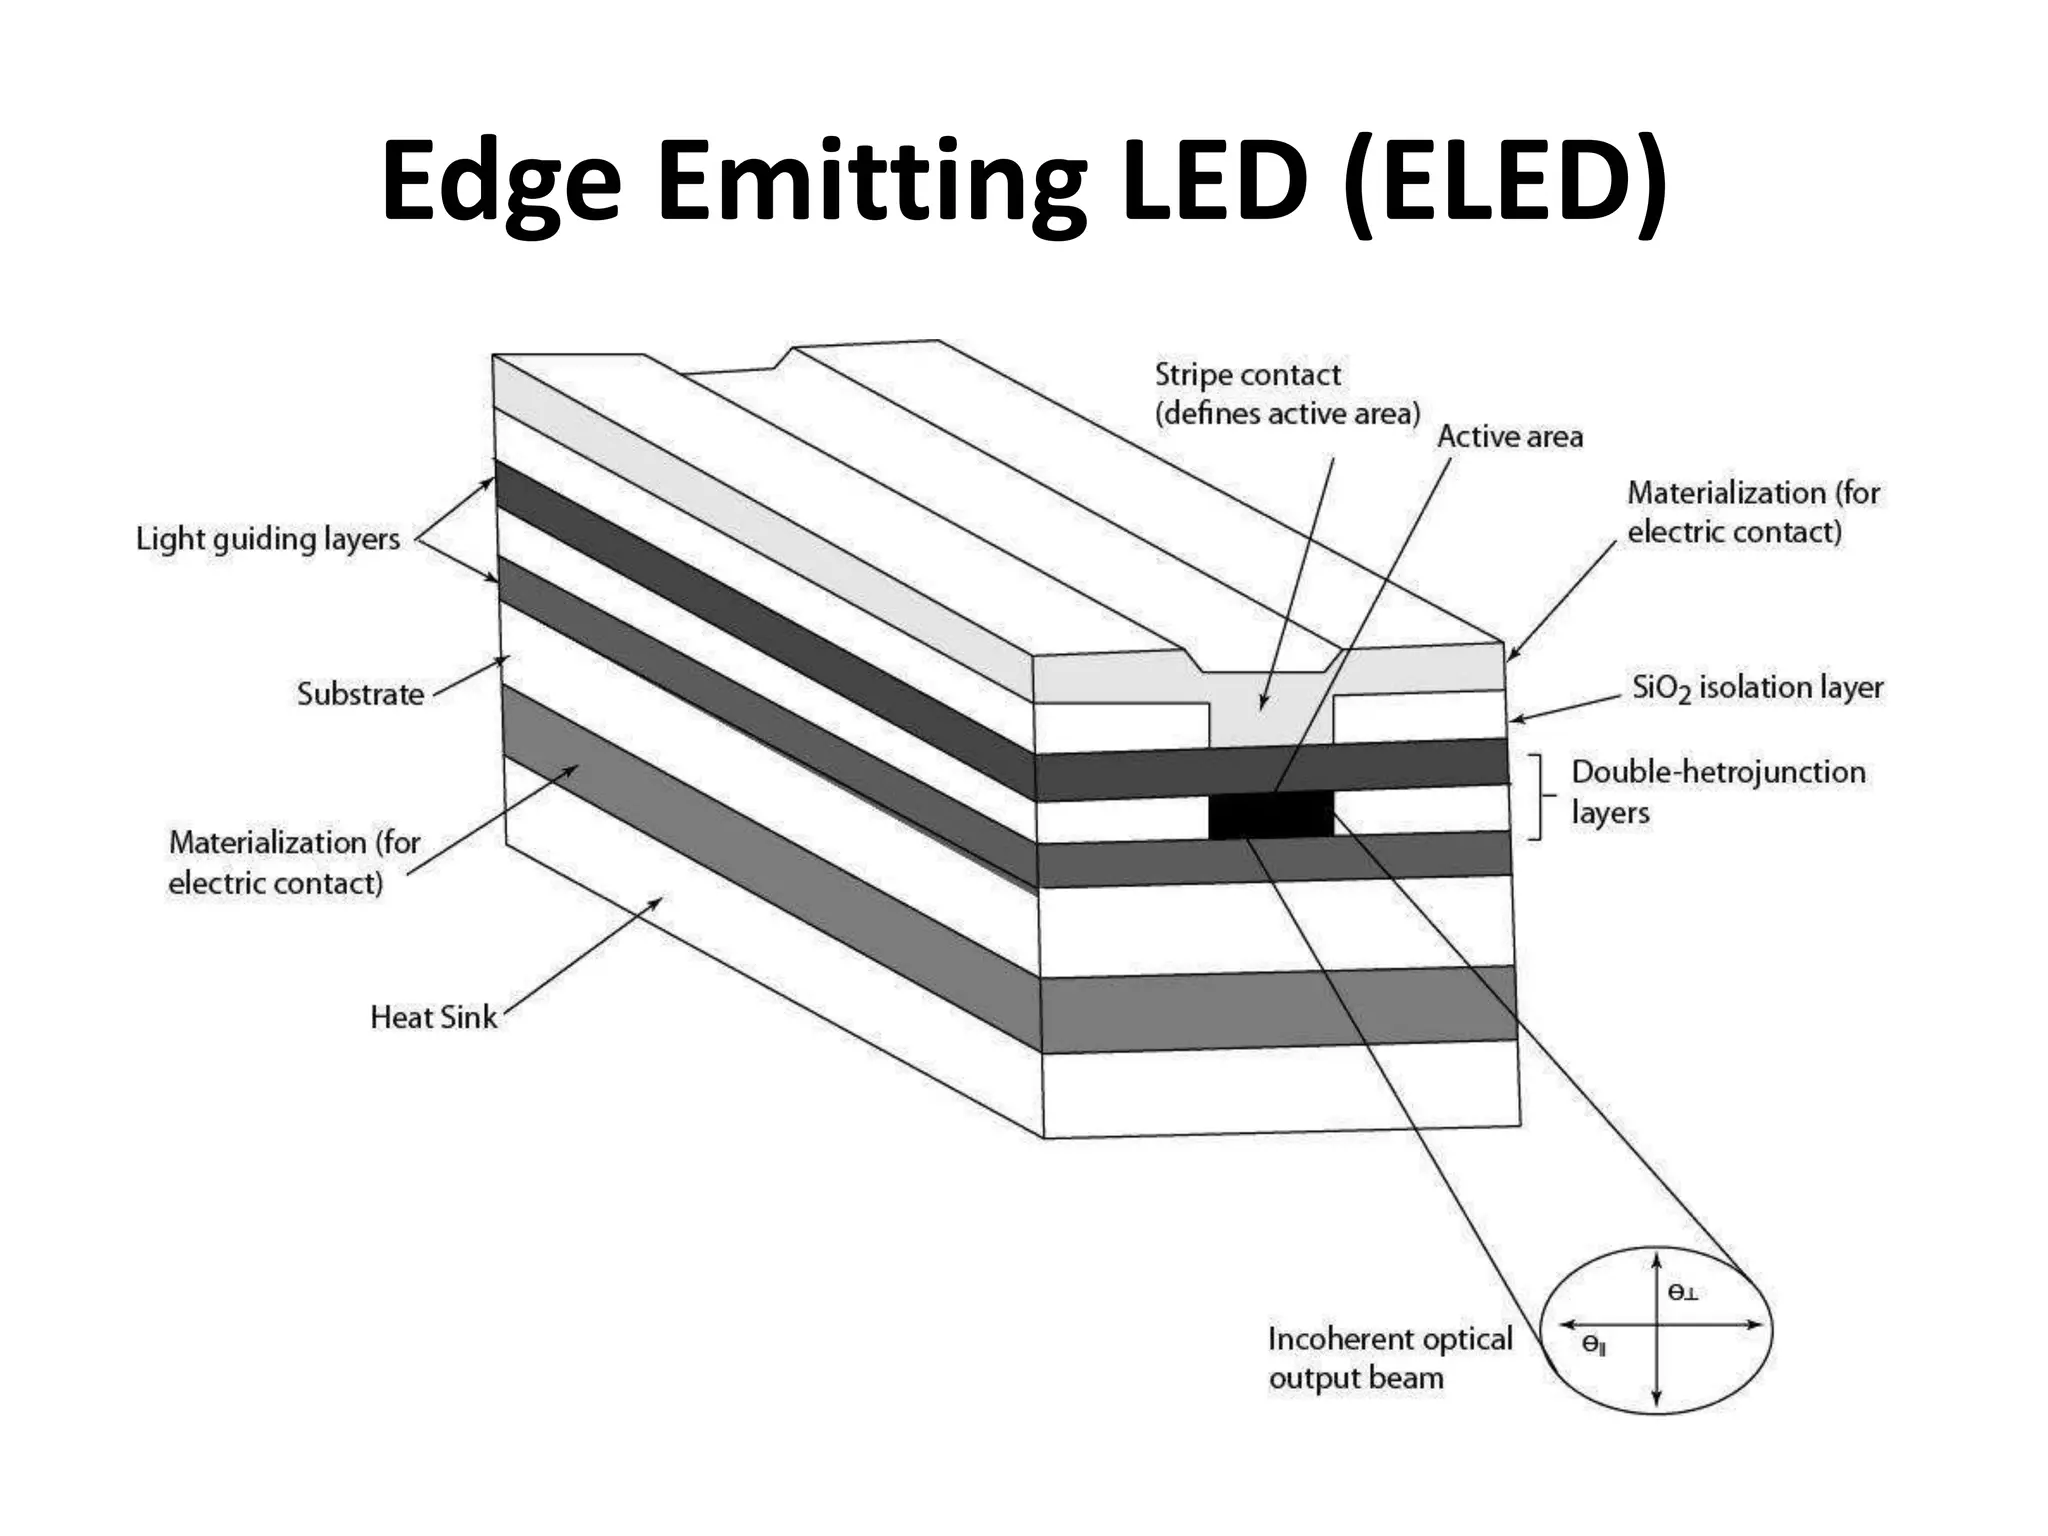
\includegraphics[width=0.6\linewidth]{Dfo/dfo7.png}
%\caption{Estrucura de un LED de emisión lateral.}
%\end{figure}
%\section{Láser}
%\begin{itemize}
%\item \textbf{Luz coherente}: La luz coherente se refiere a una luz que tiene una fase constante en el tiempo y en el espacio. Las ondas de luz coherentes tienen una relación fija entre las crestas y los valles de las ondas, lo que resulta en un patrón de interferencia bien definido. En la fibra óptica, la luz coherente se utiliza en aplicaciones como la transmisión de señales de comunicación de larga distancia y la interferometría, donde se requiere la interferencia precisa de las ondas de luz para mediciones precisas.
%\item \textbf{Luz incoherente}: La luz incoherente es una luz en la que la fase de las ondas varía de manera aleatoria en el tiempo y el espacio. No hay una relación fija entre las crestas y los valles de las ondas de luz incoherentes, lo que resulta en una interferencia destructiva promediada a lo largo del tiempo. En la fibra óptica, la luz incoherente se utiliza en aplicaciones como la iluminación general, donde la uniformidad de la iluminación es más importante que la interferencia de las ondas de luz.
%\end{itemize}
%\begin{figure}[H]
%\centering
%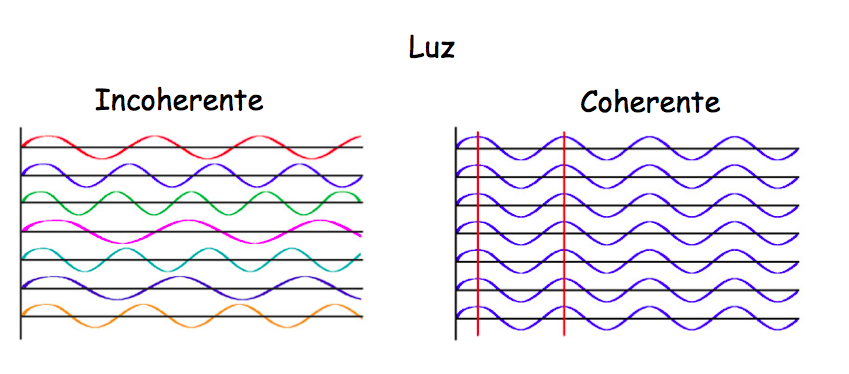
\includegraphics[width=0.6\linewidth]{Dfo/dfo8.png}
%\caption{Luz coherente e incoherente.}
%\end{figure}
%Siguiendo con los \textbf{diodos láser}, estos son fuentes de luz amplificada coherente. Basa en una estructura de uniones de material semiconductor del tipo p-n, formando una cavidad óptica resonante  (del tipo Fabry-Perot) para proporcionar la realimentación de fotos y aumentar la emisión estimulada.
%\begin{definition}[Cavidad óptica resonante]
%Una cavidad óptica resonante es una estructura diseñada para mantener y amplificar la luz que se propaga en su interior. Consiste en dos o más superficies reflectantes, como espejos, que forman una configuración en la que la luz se refleja repetidamente entre ellos.\\
%Cuando la luz ingresa a la cavidad óptica resonante, parte de ella se refleja en las superficies reflectantes y parte se transmite a través de ellas. La luz reflejada se superpone y se refuerza a medida que atraviesa la cavidad una y otra vez, generando una onda estacionaria de luz dentro de la cavidad. Esto crea modos de resonancia, que son longitudes de onda específicas en las cuales la luz se amplifica y se mantiene confinada en la cavidad durante un tiempo más largo.\\
%La característica principal de una cavidad óptica resonante es su capacidad para aumentar la intensidad de la luz en ciertas longitudes de onda. La amplificación se logra al reflejar repetidamente la luz en las superficies reflectantes, lo que permite que la luz pase múltiples veces a través del medio activo de la cavidad, como un material láser.
%\end{definition}
%\begin{figure}[H]
%\centering
%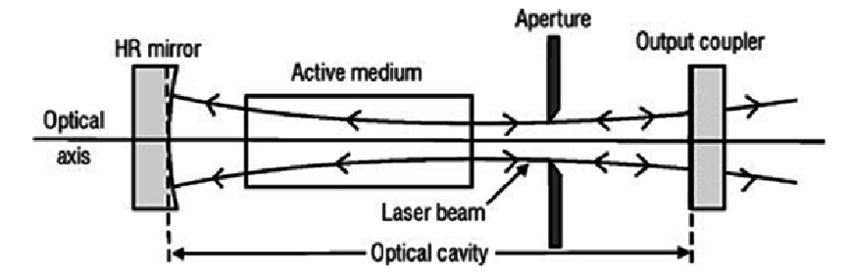
\includegraphics[width=0.6\linewidth]{Dfo/dfo9.png}
%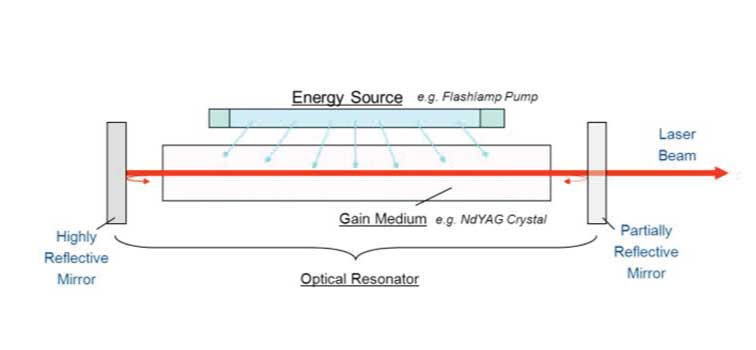
\includegraphics[width=0.6\linewidth]{Dfo/dfo10.png}
%\caption{Cavidad óptica resonante.}
%\end{figure}
%%\subsection{Estructuras de láseres}
%\subsection{Láser guiado por ganancia}
%Estructura de geometría de franjas donde la distribución de modos ópticos a lo  largo del plano de la unión es determinado por la ganancia óptica de la cavidad, por lo general proporcional a una emisión múltimodo.\\
%En un láser convencional, la retroalimentación necesaria para la amplificación de la luz proviene de un par de espejos colocados en los extremos de la cavidad láser. Sin embargo, en un láser guiado por ganancia, la \textbf{retroalimentación} se logra a través de una guía de ondas óptica que contiene el \textbf{medio activo} de ganancia.\\
%El medio activo de ganancia puede ser un material semiconductor \textbf{dopado}, como un láser de semiconductor, o un material amplificador de fibra óptica. Este medio activo proporciona la ganancia necesaria para amplificar la luz a medida que se propaga a través de él. La guía de ondas óptica, por otro lado, se utiliza para confinar y direccionar el haz láser. Puede ser una guía de ondas de semiconductor, una fibra óptica, una guía de ondas plana o cualquier otra estructura que sea capaz de guiar la luz en la dirección deseada. La combinación de la ganancia del medio activo y la guía de ondas óptica permite que el láser guiado por ganancia genere un haz láser altamente \textbf{direccional} y \textbf{coherente}. La retroalimentación se logra mediante múltiples reflexiones internas dentro de la guía de ondas, lo que amplifica la luz en el medio activo y produce una emisión láser.
%\begin{figure}[H]
%\centering
%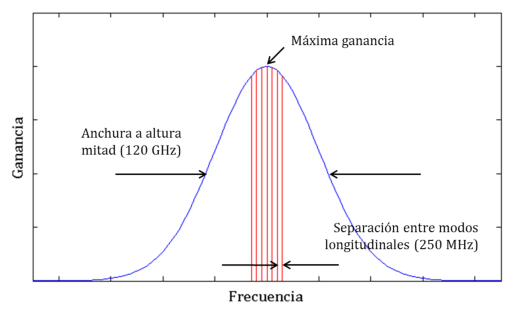
\includegraphics[width=0.6\linewidth]{Dfo/dfo11.png}
%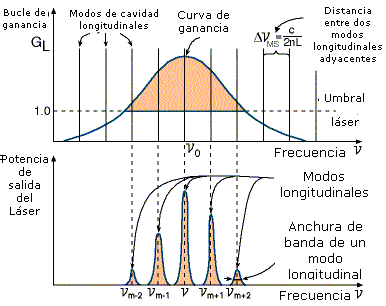
\includegraphics[width=0.6\linewidth]{Dfo/dfo12.png}
%\caption{Espectro de un láser de ganancia guiada.}
%\end{figure}
%\begin{definition}[Distancia entre los modos longitudinales adyacentes]
%Esta distancia se conoce como longitud de onda de modo libre (Free Spectral Range, FSR) y se calcula utilizando la siguiente fórmula:
%\begin{equation}
%\delta v_{ms}=\frac{c}{2nL}
%\end{equation}
%Donde:
%\begin{itemize}
%\item c: Velocidad de la luz ($3\basedec{10} m/s$). (m/s)
%\item L: Longitud efectiva de la cavidad láser. (m)
%\item n: Indice de refacción de el medio.
%\end{itemize}
%\end{definition}
%\begin{definition}[Anchura total a la mitad de la máxima amplitud]
%Es la distancia entre los dos puntos en los cuales el valor de la función es igual a la mitad de su valor máximo. Es decir, es la distancia entre los dos puntos donde la función alcanza la mitad de su amplitud máxima. El FWHM se utiliza para \textbf{cuantificar} la anchura de una función y proporciona información sobre la resolución, la dispersión o la característica de ancho de una distribución. En general, cuanto más estrecho sea el FWHM, más concentrada estará la distribución alrededor de su valor máximo, y cuanto más amplio sea el FWHM, más extendida estará la distribución.
%\begin{center}
%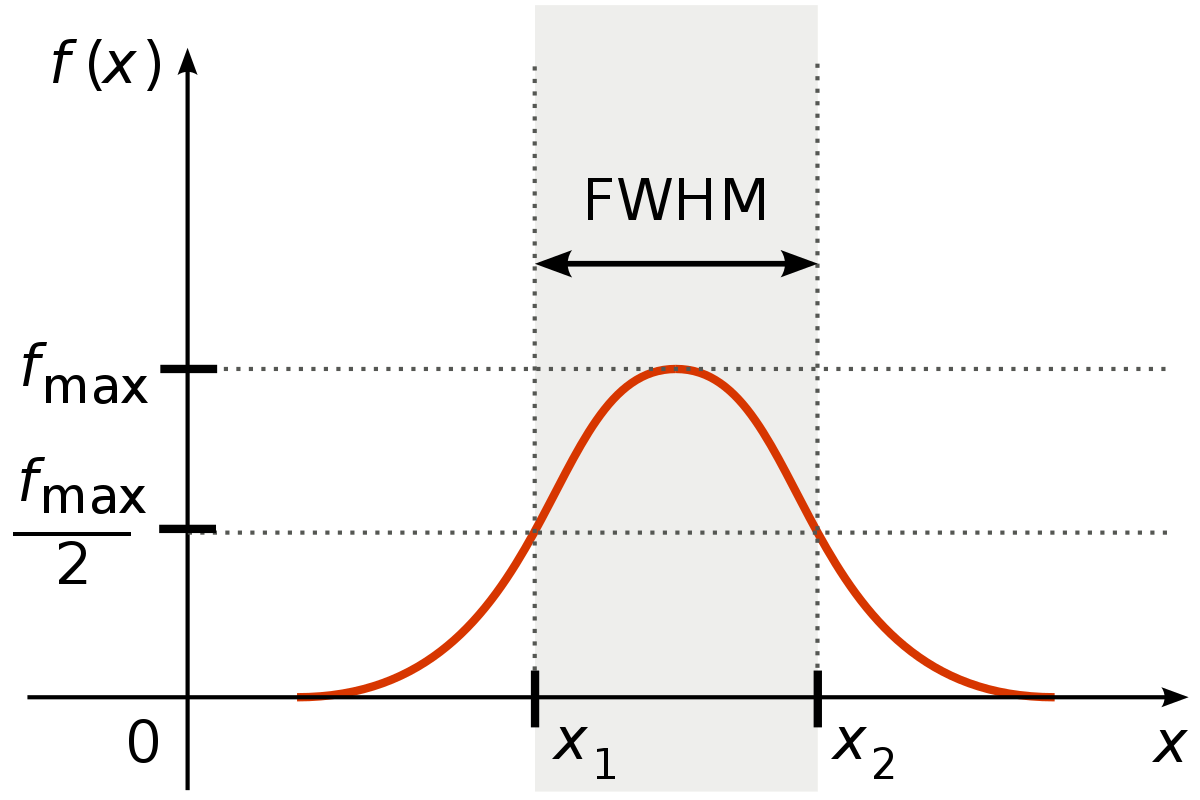
\includegraphics[width=0.6\linewidth]{Dfo/dfo13.png}
%\end{center}
%Si se asume una distreibución Gaussiana, donde $\sigma$ es la varianza de la distribución Gaussiana, FWHM puede ser calculado como:
%\begin{equation}
%FWHM=2\sigma\sqrt{2\ln 2}=2.35\sigma
%\end{equation}
%\begin{center}
%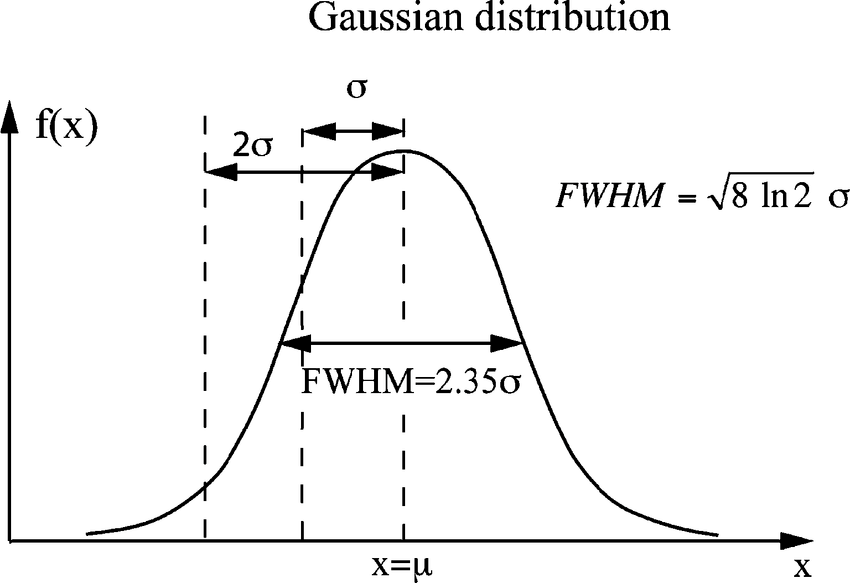
\includegraphics[width=0.6\linewidth]{Dfo/dfo14.png}
%\end{center}
%\end{definition}
%\subsection{Láser Monomodo}
%Son utilizadas para comunicaciones de largo alcance, con un espectro muy angosto con la emisión de un único modo longitudinal y transversal. Se busca eliminar o suprimir los modos adyacentes para lograr una operación de un solo modo. Algunos tipos son:
%\begin{itemize}
%\item Láser de cavidad vertical (VCSEL): Son láseres monomodo que emiten la luz perpendicularmente a la superficie del dispositivo. Son ampliamente utilizados en aplicaciones de comunicaciones ópticas de corta distancia, como redes de área local (LAN) y enlaces de fibra óptica de corto alcance.
%\item Láser de diodo monomodo: Los láseres de diodo monomodo son dispositivos láser que utilizan un diodo semiconductor como medio activo y se diseñan para operar en un único modo longitudinal. Son ampliamente utilizados en aplicaciones de comunicaciones ópticas, medicina, investigación y otros campos.
%\item Láser de fibra monomodo: Los láseres de fibra monomodo utilizan una fibra óptica como medio de ganancia para generar un haz láser monomodo. La fibra óptica guía la luz de manera efectiva en un único modo, lo que permite una alta calidad de haz y una estrecha anchura espectral. Estos láseres son ampliamente utilizados en aplicaciones de telecomunicaciones, medicina, sensores ópticos y láseres de alta potencia.
%\item Láser de cavidad externa: Los láseres de cavidad externa utilizan una configuración en la que se acopla un láser de diodo o de fibra a una cavidad externa, como una resonador de Fabry-Perot o una cavidad de anillo. Esto permite controlar y seleccionar un único modo longitudinal para la emisión láser. Estos láseres se utilizan en aplicaciones que requieren una alta precisión espectral, como la espectroscopia y la metrología.
%\end{itemize}
%Estructura que proporciona una re-alimentación selectiva de frecuencia de manera que la pérdida de la cavidad es diferente para variar modos longitudinales. La emisión de la luz contiene un solo modo longitudinal.
%\subsubsection{Láser DFB y DBR}
%\begin{enumerate}
%\item \textbf{Láser de retroalimentación distribuida} (\textit{DFB, por sus siglas en inglés - Distributed Feedback Laser}): Un láser DFB es un tipo de láser de diodo que utiliza una rejilla de retroalimentación incorporada en la estructura del dispositivo. Esta rejilla de retroalimentación tiene una periodicidad precisa y se utiliza para proporcionar una retroalimentación óptica que favorece la emisión de luz en un único modo longitudinal y en una estrecha banda espectral. El láser DFB se caracteriza por su estabilidad en frecuencia y alta calidad de haz. Se utiliza en aplicaciones de comunicaciones ópticas de larga distancia, como en sistemas de transmisión de fibra óptica de alta velocidad.
%\item \textbf{Láser de reflector de banda distribuida} (\textit{DBR, por sus siglas en inglés - Distributed Bragg Reflector Laser}): Un láser DBR es otro tipo de láser de diodo que utiliza reflectores de banda distribuida para proporcionar retroalimentación óptica. Los reflectores de banda distribuida son estructuras formadas por capas alternas de materiales con diferentes índices de refracción. Estos reflectores actúan como espejos ópticos selectivos en un rango de longitudes de onda específico. Al ajustar la corriente de inyección del láser DBR, se puede sintonizar la longitud de onda de emisión. El láser DBR se utiliza en aplicaciones de comunicaciones ópticas, espectroscopia, sensores ópticos y otras áreas donde se requiere una sintonización precisa de la longitud de onda.
%\end{enumerate}
%\begin{figure}[H]
%\centering
%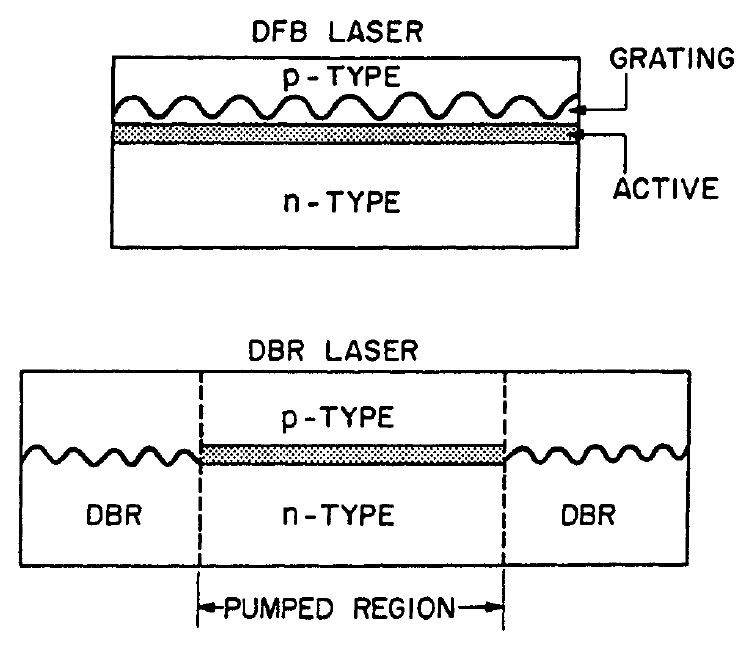
\includegraphics[width=0.8\linewidth]{Dfo/dfo15.png}
%\caption{Láseres DFB y DBR.}
%\end{figure}
%\begin{figure}[H]
%\centering
%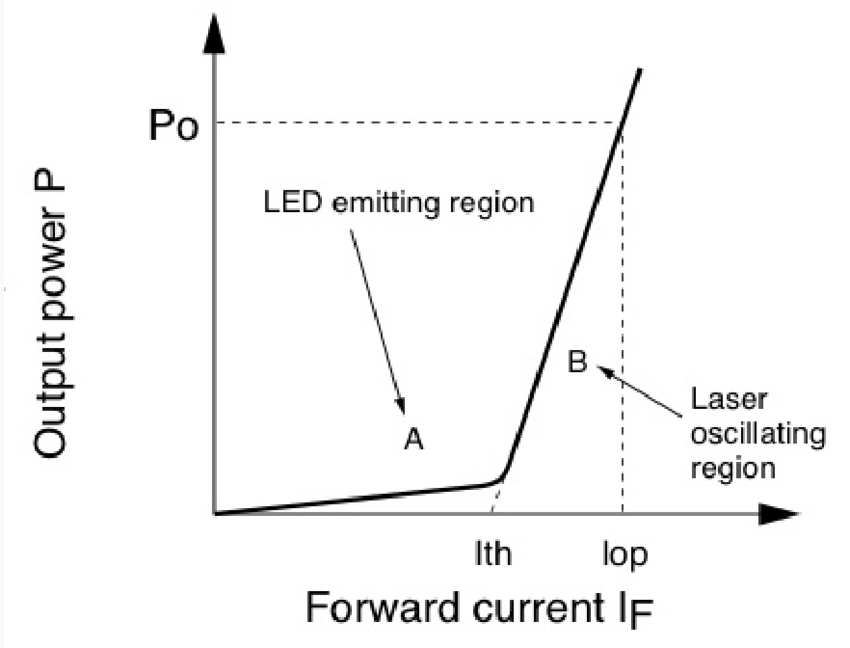
\includegraphics[width=0.8\linewidth]{Dfo/dfo16.png}
%\caption{Características de los diodos láser.}
%\end{figure}
%En un láser, la corriente de inyección es el factor determinante para controlar la emisión de luz. A medida que se aumenta la corriente de inyección, se incrementa la población de portadores de carga en el material activo del láser, lo que conduce a una mayor emisión estimulada de fotones y, por lo tanto, a un aumento en la potencia de salida. \\
%La gráfica de potencia de salida vs corriente generalmente muestra un comportamiento característico. Inicialmente, a bajas corrientes, la potencia de salida aumenta gradualmente a medida que se inyecta más corriente en el láser. Luego, a medida que se alcanza un cierto punto, la potencia de salida comienza a aumentar más rápidamente, alcanzando un máximo en un punto óptimo de operación conocido como "punto de máxima potencia". Más allá de este punto, la potencia de salida puede estabilizarse o incluso disminuir debido a fenómenos como la saturación del medio activo o el aumento de la disipación de calor. \\
%La gráfica de potencia de salida vs corriente es esencial para determinar el rango de corrientes de funcionamiento óptimo del láser. Permite identificar el punto de máxima potencia, donde el láser opera de manera más eficiente y se obtiene la máxima potencia de salida. También ayuda a determinar los límites de operación del láser, como corrientes mínimas y máximas, y proporciona información sobre la estabilidad y el comportamiento del láser en diferentes condiciones.
%\subsection{VCSEL}
%\begin{figure}[H]
%\centering
%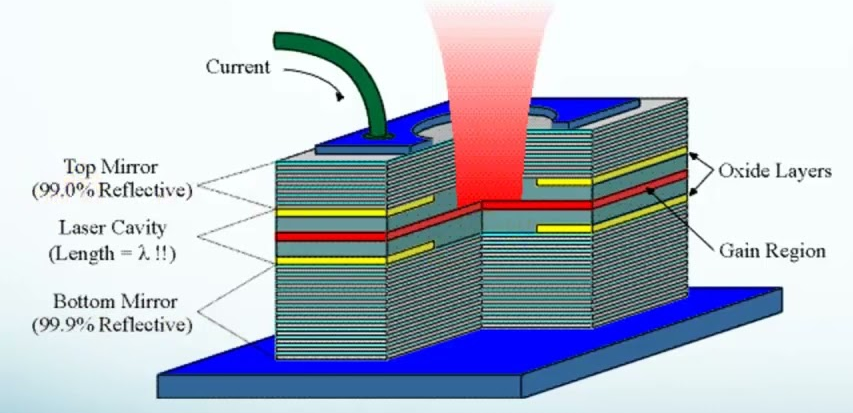
\includegraphics[width=0.6\linewidth]{Dfo/dfo17.png}
%\caption{Vertical-Cavity Surface-Emitting Laser}
%\end{figure}
%Un VCSEL (Vertical-Cavity Surface-Emitting Laser, por sus siglas en inglés) es un tipo de láser semiconductor que emite luz perpendicularmente a la superficie del dispositivo. A diferencia de los láseres de borde, que emiten luz a lo largo de un borde de la unión p-n, los VCSEL emiten luz a través de la parte superior e inferior de la estructura semiconductor. El funcionamiento básico de un VCSEL se basa en la creación de una cavidad óptica resonante vertical dentro del dispositivo. La estructura del VCSEL consta de múltiples capas de materiales semiconductores, como arseniuro de galio (GaAs) y arseniuro de aluminio (AlAs), que forman una estructura de espejo de banda distribuida. Estos espejos se utilizan para proporcionar retroalimentación óptica y formar la cavidad resonante. En el centro de la estructura del VCSEL se encuentra una capa activa, que generalmente consiste en una capa de material semiconductor dopada con impurezas para crear una unión p-n. Cuando se aplica una corriente eléctrica a través de la unión p-n, se inyectan portadores de carga (electrones y huecos) en la capa activa. Estos portadores se recombinan en la región activa y generan emisión de luz. La geometría vertical del VCSEL permite que la luz emitida se acople eficientemente en el modo transversal fundamental de la cavidad resonante. La longitud de onda de la luz emitida está determinada por la separación entre los espejos de banda distribuida y las propiedades de los materiales utilizados.\\
%Una ventaja clave de los VCSEL es su facilidad para fabricar matrices bidimensionales de dispositivos, lo que permite la construcción de módulos de emisión de alta densidad. Además, los VCSEL tienen una alta eficiencia de acoplamiento óptico, una alta velocidad de modulación y una emisión de luz con una distribución de haz circular y simétrica.
%\subsection{Diagrama de ojo}
%%Diagrama de ojo
%Los dispositivos LED y LASER deben cumplir ciertos parámetros generales para su uso en los sistemas ópticos, que deben orientarse a:
%\begin{itemize}
%\item Definir el comportamiento respecto a la conversión electro-óptica
%\item Adecuar las características radiométricas de los dispositivos de acuerdo con el portador físico (fibra óptica).
%\item Diseñar circuitos de excitación idóneos con respecto a la naturaleza del tipo emisor.
%\end{itemize}




%------------------------------------------------------------
\end{document}
%----------------------------------------------------------------------------------------
